
\section{Tabeller}

\begin{center}
	\begin{tabular}{| m{4cm} |m{4cm} |m{4cm} |} 
\hline
	\multicolumn{3}{|c|}{\textbf{\cellcolor[HTML]{D5D5D5}Oversikt over laboppgaver}} \\
\hline
\hline
\rowcolor [HTML]{D5D5D5}
Finn eller beregn 		&Verdi				&Kommentar							\\ \cline{1-3}
Ib - belastningsstrøm		&				&								\\ \cline{1-3}
In – Nominell størrelse vern	&				&$Ib \leq In$							\\ \cline{1-3}
Karakteristikk			&				&								\\ \cline{1-3}
Referanseinstallasjonsmetode	&				&Figur D.1 side 118						\\ \cline{1-3}
2- eller 3-leder		&				&								\\ \cline{1-3}
PVC eller PEX			&				&								\\ \cline{1-3}
Strømføringsevne (Iz) 		&				&Tabell 6 side 81						\\ \cline{1-3}
Tverrsnitt			&				&								\\ \cline{1-3}
Omgivelsestemperatur		&$Temp:\hskip 1cm k_{temp}:$	&Tabell D.1 side 117						\\ \cline{1-3}
Nærføring			&$Antall:\hskip 0.9cm k_{ner}:$		&Tabell D.2 side 119					\\ \cline{1-3}
Ny Strømføringsevne (Iz)	& 				&$I_z\cdot k_{temp} \cdot k_{ner}$ 				\\ \cline{1-3}
Krav 1				&				&$Ib \leq In \leq Iz$						\\ \cline{1-3}
Krav 2				&				&$I2 \leq 1,45 \cdot Iz$					\\ \cline{1-3}
Motstand leder ($R_l$) 		&				&$R_l= \dfrac {\rho \cdot l \cdot \sqrt{3} \cdot cos\phi}{A}$ 	\\ \cline{1-3}
Motstand ved 70°C ($R_{l_{70}}$)	&				&$R_{l_{70}}=R_l \cdot 1,2$				\\ \cline{1-3}
Spenningsfall $\Delta U$	&				&$\Delta U=R_{l_{70}} \cdot I_b$				\\ \cline{1-3}
Spenningsfall \%  		&				&$\Delta U_{i \%}= \dfrac{ \Delta U}{U} \cdot 100\%$		\\ \cline{1-3}
Vurdering spenningsfall 	&				&								\\ \cline{1-3}
Kontroller at vernet ikke slår ut på startstrømmen 	& 	&$I_{start}< I_4$						\\ \cline{1-3}
Ikmin på siste punkt		& 				&								\\ \cline{1-3}
Vernets I5			& 				&								\\ \cline{1-3}
Løser vernet ut momentant ved kortslutning		& 	&$I_5\leq Ik_{min}$ 						\\ \cline{1-3}
Hvor lang tid tar det før vernet løser ut		& 	& 								\\ \cline{1-3}
Kontroller maksimal kabellengde 			&	&Tabell 10 side 102 						\\ \cline{1-3}
Tåler vernet største kortslutning 			& 	&$Ik_{maks} \leq I_{cu}$ 					\\ \cline{1-3}
Hvor lenge tåler kabelen kortslutningen  		& 	&D.4 side 121  $t=(k \cdot \frac{S}{I})^2$ 			\\ \cline{1-3}
Løser sikringen ut før kabelen blir ødelagt? 		& 	&$0,1s < t < 5s$ 						\\ \cline{1-3}


		
\end{tabular}
\end{center}



	
\newpage
\includegraphics[width=1\textwidth]{002.eps}
\vfil \eject
\includegraphics[angle=90,height=1\textheight]{./chemistry12.eps}
\vfil \eject
\includegraphics[width=1\textwidth]{calibrate03.eps}
\includegraphics[width=1\textwidth]{calibrate04.eps}
\includegraphics[width=0.5\textwidth]{current09.eps}
\includegraphics[width=0.5\textwidth]{current10.eps}
\includegraphics[width=0.5\textwidth]{current11.eps}
\includegraphics[width=0.5\textwidth]{current12.eps}
\includegraphics[width=0.5\textwidth]{current13.eps}
\includegraphics[width=0.5\textwidth]{current29.eps}
\includegraphics[width=0.5\textwidth]{current30.eps}
\includegraphics[width=0.5\textwidth]{current31.eps}
\includegraphics[width=1\textwidth]{plc_048.eps}
\includegraphics[width=1\textwidth]{plc_052.eps}
\includegraphics[width=1\textwidth]{pressure76.eps}
